\documentclass[12pt]{article}
\usepackage{graphicx}
\graphicspath{ {experiments/} }

\title{Computer Network Lab 3 Report}
\author{
    {\em Chao Xin} \\
    {\tt cxin@andrew.cmu.edu}
    \and
    {\em Yimin Liu} \\
    {\tt yiminliu@andrew.cmu.edu}
}
\date{}

\begin{document}

\maketitle

\section{Experiments}

We experimented the proxy on the dumbbell topology with $\alpha$ = 0.1 0.5 and 0.9. Here is the experiment data we get.\\

\begin{figure}
\centering
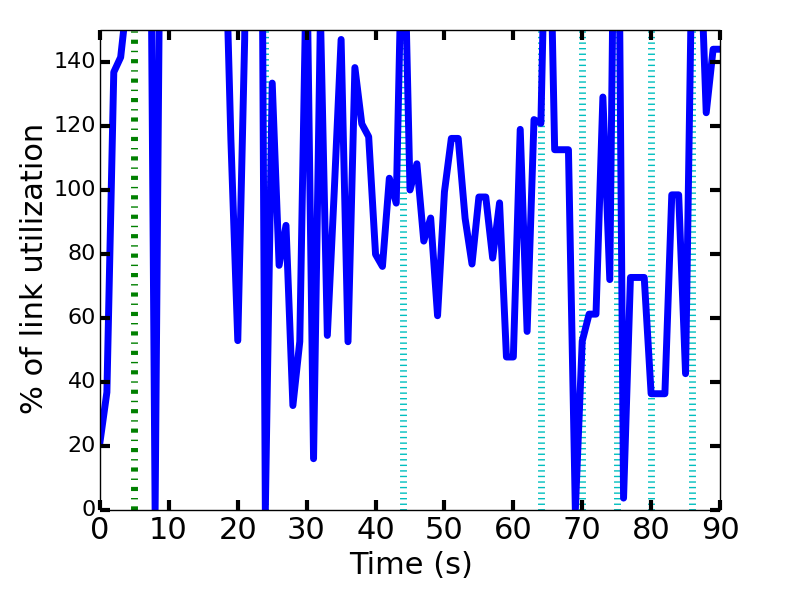
\includegraphics[scale = 0.75]{exp1/utilization.png}
\caption{Utilization for $\alpha$ = 0.1}
\end{figure}

\begin{figure}
\centering
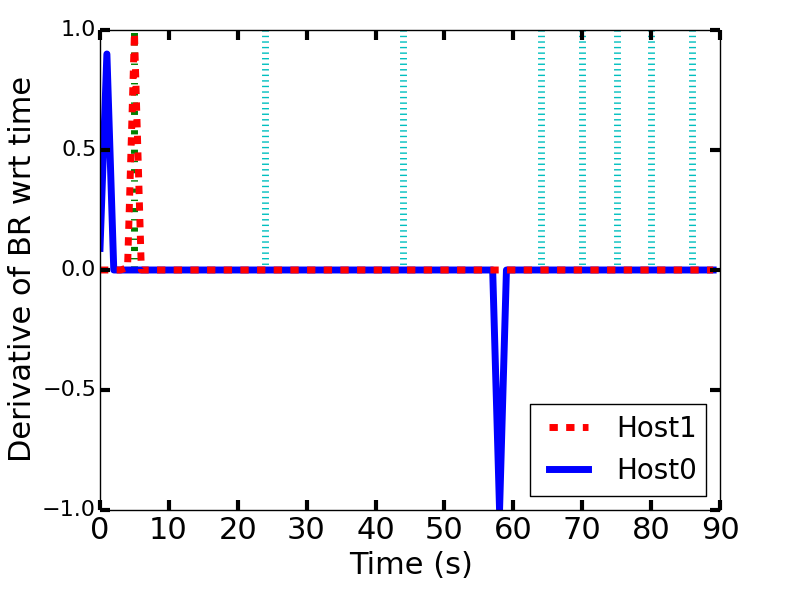
\includegraphics[scale = 0.75]{exp1/smoothness.png}
\caption{Smoothness for $\alpha$ = 0.1}
\end{figure}

\begin{figure}
\centering
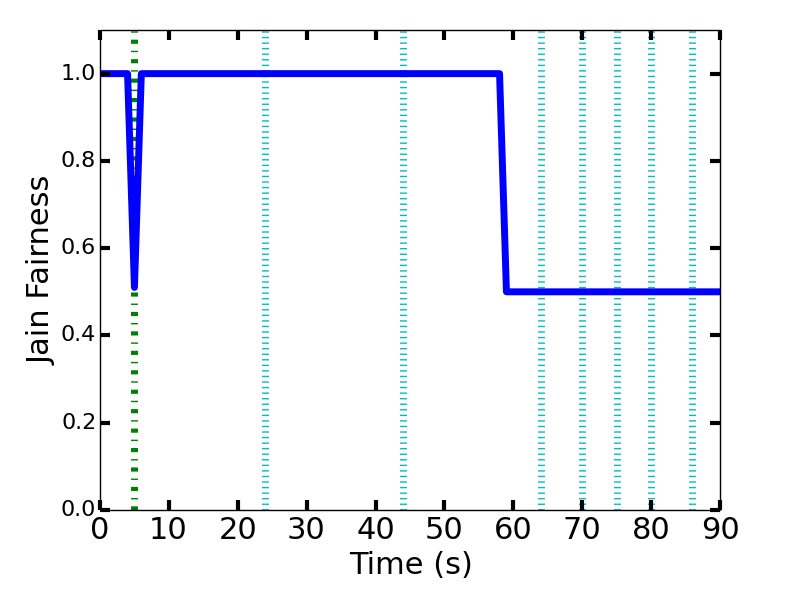
\includegraphics[scale = 0.75]{exp1/fairness.png}
\caption{Fairness for $\alpha$ = 0.1}
\end{figure}

\begin{figure}
\centering
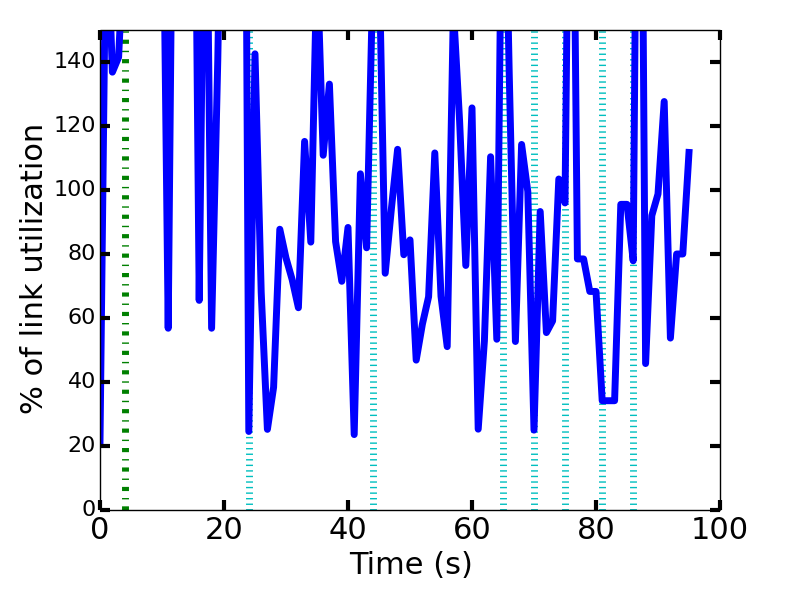
\includegraphics[scale = 0.75]{exp2/utilization.png}
\caption{Utilization for $\alpha$ = 0.5}
\end{figure}

\begin{figure}
\centering
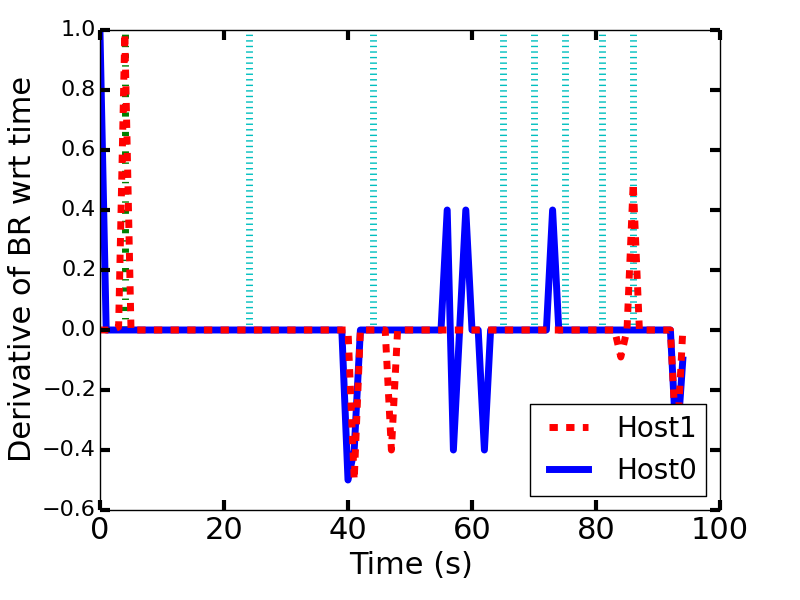
\includegraphics[scale = 0.75]{exp2/smoothness.png}
\caption{Smoothness for $\alpha$ = 0.5}
\end{figure}

\begin{figure}
\centering
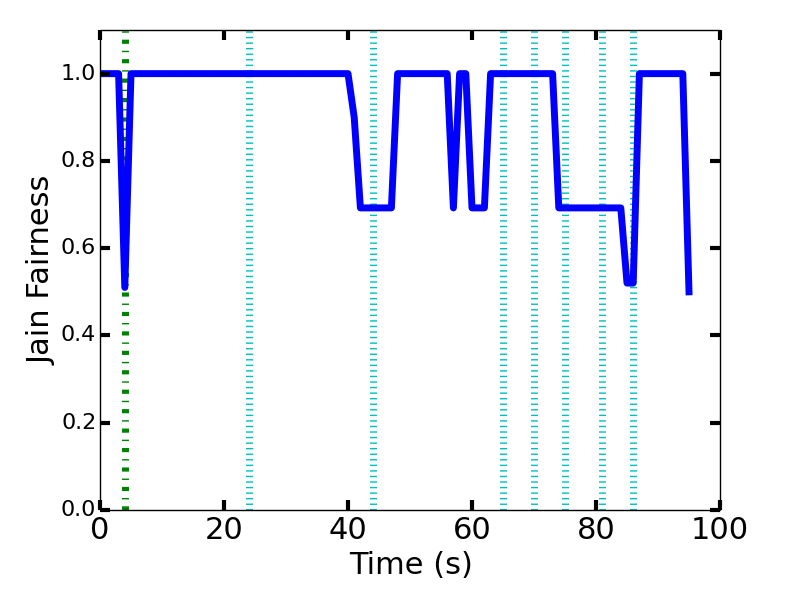
\includegraphics[scale = 0.75]{exp2/fairness.png}
\caption{Fairness for $\alpha$ = 0.5}
\end{figure}

\begin{figure}
\centering
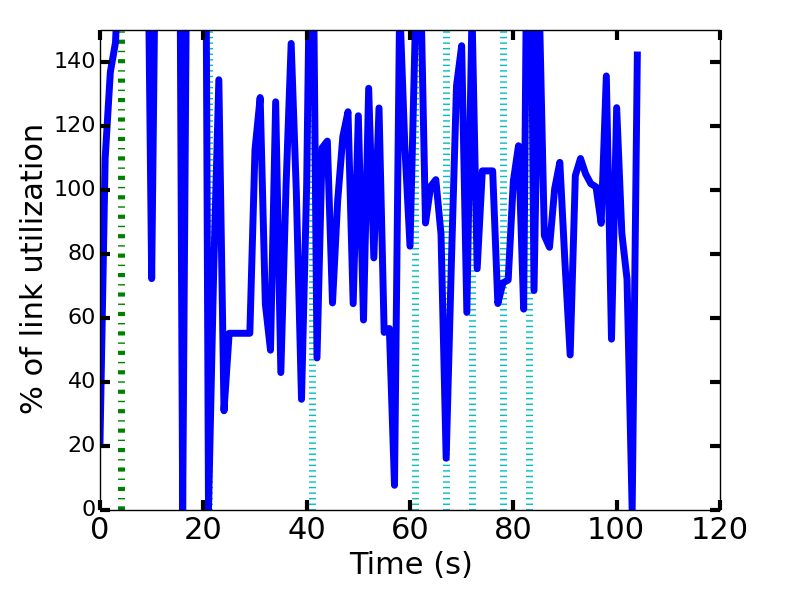
\includegraphics[scale = 0.75]{exp3/utilization.png}
\caption{Utilization for $\alpha$ = 0.9}
\end{figure}

\begin{figure}
\centering
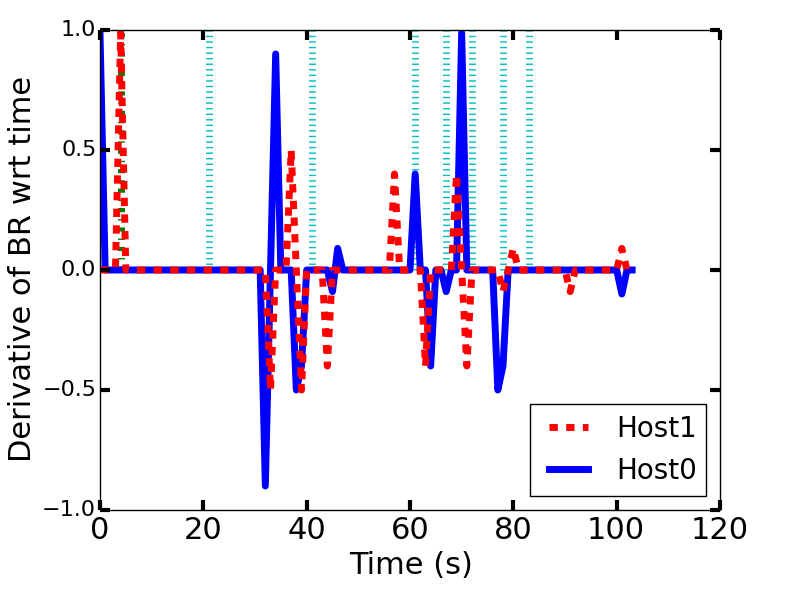
\includegraphics[scale = 0.75]{exp3/smoothness.png}
\caption{Smoothness for $\alpha$ = 0.9}
\end{figure}

\begin{figure}
\centering
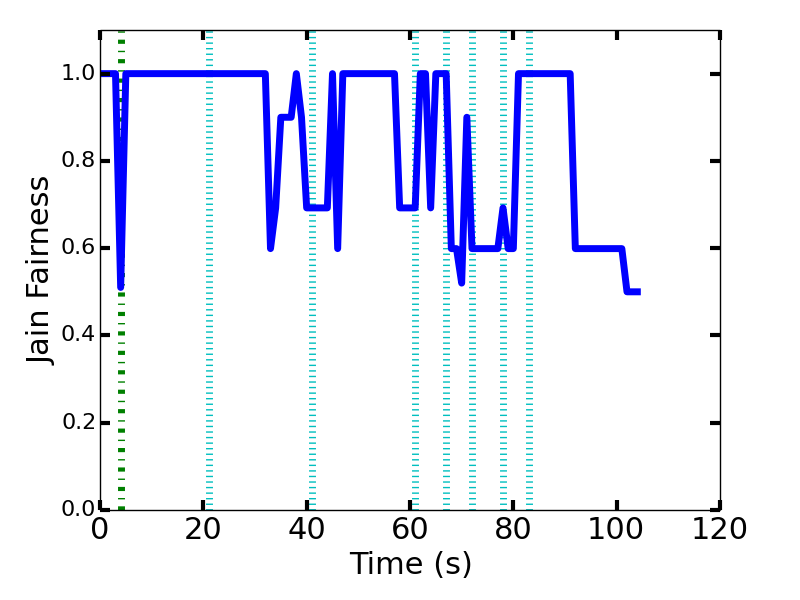
\includegraphics[scale = 0.75]{exp3/fairness.png}
\caption{Fairness for $\alpha$ = 0.9}
\end{figure}

\section{Analysis}

It can be seen from the plot that lower $\alpha$ can achieve higher smoothness. While higher $\alpha$ can achieve better fairness. The utilization varies a lot and obvious patterns can't be found.

\end{document}